%&latex
%
\documentclass[../template.tex]{subfiles}
\begin{document}

\lesson{4}{21/10/19}
\section{Wiener's integral}
Consider an \textit{unconstrained} Brownian particle, moving on the real line, starting in $x_0$ at $t_0$. By solving the diffusion equation we found that the probability of finding the particle in $[x,x+\dd{x}]$ at time $t > t_0$ is given by the \textbf{propagator}:
\begin{align} \nonumber
  \mathbb{P}\{x(t) \in [x,x+\dd{x}]|x(t_0) = x_0\} &=  W(x,t|x_0,t_0) \dd{x} = \\
  &= \frac{1}{\sqrt{4 \pi D (t-t_0) }} \exp\left(-\frac{(x-x_0)^2}{4 D (t-t_0)} \right) \dd{x} \label{eqn:propagator}
\end{align}  
By integrating (\ref{eqn:propagator}) we can then find the probability of finding the particle inside an interval $[A,B]$ at time $t$: 
\begin{align*}
    \mathbb{P}\{x(t) \in [A,B]|x(t_0) = x_0\} = \int_A^B \dd{x} W(x,t|x_0, t_0) \qquad t>t_0
\end{align*}
We are now interested in computing the expected value $\langle f \rangle$  of \textbf{functionals} $f$ of the trajectory, i.e. of quantities depending on several (or all) points of the trajectory $x(\tau)$ of a Brownian particle. 

\begin{itemize}
    \item The simplest example is the \textbf{correlation function}, which is defined as the product of the particle's position at two different times $t_1 < t_2$:
    \begin{align*}
        f(\{x(t_1), x(t_2)\}) = x(t_1) x(t_2) \quad t_1 < t_2
    \end{align*} 

    \item A more general (and difficult) case is given by a function of the \textit{entire} trajectory, such as:
    \begin{align*}
        f(\{x(\tau)\colon 0 < \tau \leq \tau\}) = g\left(\int_0^t x(\tau) a(\tau) \dd{\tau}\right)\qquad a,\>g\colon \mathbb{R} \to \mathbb{R}
    \end{align*}
\end{itemize}

\subsection{Functions of a discrete number of points}
Let's start from the simplest case, and consider the \textbf{correlation function}:
\begin{align*}
    f(\{x(t_1), x(t_2)\}) = x(t_1) x(t_2) \qquad t_1 < t_2
\end{align*}
To compute $\langle f \rangle$ we will need the \textit{joint probability distribution} $g(x_1,x_2)$ that gives the probability of $x(t_1)$ being \q{close to} $x_1$ \textbf{and} $x(t_2)$ \q{close to} $x_2$ \textit{for the same trajectory}. Let us denote the three events of interest:
\begin{align*}
    A &\colon \text{Particle starts in $x_0$ at $t_0$}\\
    B &\colon \text{Particle is close to $x_1$ at $t_1$ ($x(t_1) \in [x_1, x_1+\dd{x_1}]$)}\\
    C &\colon \text{Particle is close to $x_2$ at $t_2$ ($x(t_2) \in [x_2, x_2+\dd{x_2}]$)} 
\end{align*}
We are interested in the joint probability $\mathbb{P}(C,B|A)$ (the order is defined by $t_2 > t_1 > t_0$). From probability theory:
\begin{align*}
    \mathbb{P}(C,B|A) = \mathbb{P}(C|B,A) \mathbb{P}(B|A)
\end{align*} 
We already now how to compute probabilities like $\mathbb{P}(B|A)$, but not like $\mathbb{P}(C|B,A)$. Fortunately, that is not needed.

Recall, in fact, that Brownian motion is a \textit{Markovian process}, meaning that the \textit{future} depends only on the \textit{present state}, i.e. the particle \textit{has no memory}. So, \textbf{subsequent displacements are independent}: the probability of the particle going from $x_1$ to $x_2$ is the same whether it has started at $x_0$ or at any other point $\tilde{x}_0$. In other words, if we take the \textit{present state} as the particle being in $x_1$ at $t_1$, the future (position at $t_2 > t_1$) depends only on that, and not on the past (position at $t_0$). So:
\begin{align*}
    \mathbb{P}(C|B,A) = \mathbb{P}(C|B)
\end{align*}             
leading to:
\begin{align*}
    \mathbb{P}(C,B|A) = \mathbb{P}(C|B) \mathbb{P}(B|A)
\end{align*}
Inserting the \textit{propagators} (\ref{eqn:propagator}):
\begin{align*}
    \dd{\mathbb{P}}_{t_1,t_2}(x_1, x_2) \equiv W(x_2,t_2|x_1,t_1) W(x_1,t_1|x_0,t_0) \dd{x_1} \dd{x_2}
\end{align*}  
This is the joint probability we need to compute $\langle f \rangle$. Of course, nothing stops us from considering $N$ \q{jumps} instead of only $2$:
\begin{align} \nonumber
    \dd{\mathbb{P}}_{t_1,\dots,t_n}(x_1,\dots,x_n |x_0,t_0) &\equiv W(x_n, t_n |x_{n-1},t_{n-1}) \dots W(x_1,t_1|x_0,t_0) \dd{x_1} \dd{x_2} \dots \dd{x_n} =\\
    &= \exp\left(-\sum_{i=1}^n \frac{(x_i - x_{i-1})^2}{4 \pi D \Delta t_i} \right) \prod_{i=1}^n \frac{\dd{x_i}}{\sqrt{4 \pi D \Delta t_i}} 
    \label{eqn:ptn}
\end{align}  
Then, the average of a generic function $f(x(t_1), \dots, x(t_n))$ of the positions of the particle at times $t_1 < t_2 < \dots < t_n$ is defined as:
\begin{align*}
    \langle f(x(t_1), \dots, x(t_n)) \rangle_w = \int_{\mathbb{R}^n} f(x_1, \dots, x_n) \dd{\mathbb{P}}_{t_1, \dots, t_n} (x_1, \dots, x_n|x_0,t_0)
\end{align*}  

\subsection{Functionals of the whole trajectory}
The quantity in (\ref{eqn:ptn}) can be interpreted as the \textit{infinitesimal volume element} spanned by all the \textit{trajectories} passing through a set of \textit{tiny gates}, as represented in figure \ref{fig:gates}.

The underlying idea is that \textit{probabilities} satisfy the axioms of \textit{measures}, that is \textit{functions that assign a measure} , i.e. a generalization of \q{size}, \textit{to all sets included in a specific collection}.


\begin{figure}[H]
    \centering
    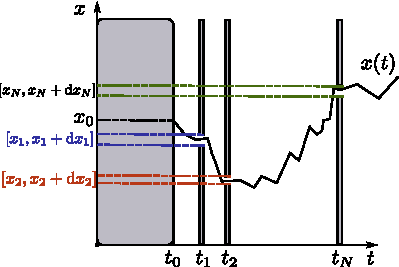
\includegraphics[width=0.7\textwidth]{Images/diffusion1.pdf}
    \caption{All trajectories that pass through the set of \textit{gates} $[x_i, x_i + \dd{x_i}]$ at times $t_i$ (such as the $x(t)$ here represented) contribute to the \textit{volume} $\dd{\mathbb{P}}_{t_1, \dots,t_n}(x_1,\dots,x_N)$ \label{fig:gates}}.
\end{figure}

We now try to formalize this idea in order to extend the results of the previous section to the case of functions depending on a \textit{infinite} number of trajectory points.

\begin{enumerate}
    \item \textbf{Space definition}. Let $T \subset \mathbb{R}$ (\textbf{index set}), denote with $\mathbb{R}^T$ the set of all functions (\textbf{stochastic processes}) $k\colon T \to \mathbb{R}$. The idea is that an element of $\mathbb{R}^T$ is a collection of \textit{random variables} indexed by $T$.
    
    In our case $T$ is a collection of time instants (e.g. $T=[0,+\infty)$) and a generic element of $\mathbb{R}^T$ is made of \textit{all the traversed points of a trajectory at times} $T$:  
    \begin{align*}
        \{x(t) \colon t \in T\} \in \mathbb{R}^T
    \end{align*}
    \item \textbf{Probability measure on finite points}. The expression in (\ref{eqn:ptn}), as observed, allows us to \textit{measure} the volumes spanned by trajectories traversing a set of gates. Let's formalize this idea. Consider a \textit{finite} set of times $T = \{t_i\}_{i=1,\dots,n}$ with $n \in \mathbb{N}, t_i \in \mathbb{R}$ and $t_1 < t_2 < \dots t_n$, each associated to a \textit{gate} $H_i = [a_i, b_i]$, with $a_i, b_i \in \mathbb{R}$ and $a_i < b_i$.        
    All the trajectories $\mathbb{R}^T$ traversing each $H_i$ at a time $t_i \in T$ span a \textbf{cylindrical set} $A$ of the form: 
    \begin{align*}
        A = \{x(t)\colon x(t_1) \in H_1, \dots, x(t_n) \in H_n\} \subset \mathbb{R}^T
    \end{align*}
    Using (\ref{eqn:ptn}) and integrating over the \textit{gates} we can define the measure of $A$-like sets as:
    \begin{align*}
        P_w(A) \equiv \int_{\mathbb{R}^n} \dd{\mathbb{P}}_{t_1,\dots,t_n} (x_1,\dots,x_n|x_0,t_0) \mathbb{I}_{H_1}(x_1) \dots \mathbb{I}_
        {H_n}(x_n)
    \end{align*}  
    where $\mathbb{I}_{H_i}(x_i)$ are \textbf{characteristic functions} of the gates:
    \begin{align*}
        \mathbb{I}_{H_i}(x) = \begin{cases}
            1 & x \in H_i\\
            0 & \text{otherwise}
        \end{cases}
    \end{align*}  
    In our case $H_i$ are just intervals, and so:
    \begin{align}
        P_w(A) \equiv \mathbb{P}_{t_1, \dots, t_n}(A) \underset{(\ref{eqn:ptn})}{=}  \int_{H_1} \dd{x_1}\int_{H_2}\dd{x_2} \cdots \int_{H_n} \dd{x_n} \prod_{i=1}^n \frac{1}{\sqrt{4 \pi D \Delta t_i}} \exp\left(-\frac{(x_i - x_{i-1})^2}{4 D \Delta t_i} \right) 
        \label{eqn:pmeas1}
    \end{align} 
    with $\Delta t_i = t_i - t_{i-1}$.
    \item \textbf{Generalization on infinite points}. Note that (\ref{eqn:pmeas1}) holds for any $n$. So, using $A$-like sets, we can construct a $\sigma$-algebra\footnote{A $\sigma$-algebra on a set $X$ is a collection $\Sigma$ of subsets of $X$ that includes $X$ itself, is closed under complement, and is closed under countable unions} $\mathcal{F}$ of $\mathbb{R}^T$. Then, by applying \textbf{Kolmogorov extension theorem} we can extend the measure $P_w$ we just found to the entire $\mathcal{F}$. 
    \item \textbf{Probability space}. We now have a set of \textit{all possible outcomes} $\mathbb{R}^T$ (in our case, all the possible trajectories that can be produced by a Brownian motion). We also have the collection of all \textit{events} $\mathcal{F}$, that is subsets of $\mathbb{R}^T$ for which is meaningful to assign a \textit{probability measure} $P_w \colon \mathcal{F} \to [0,1]$. The triad $(\mathbb{R}^T, \mathcal{F}, P_w)$ forms a \textbf{probability space}, that gives a rigorous meaning to the concept of \q{computing the probability of a trajectory}.    
\end{enumerate}
The \textbf{measure} so obtained is called \textbf{Wiener measure}, and denoted as the following:
\begin{align*}
    P_w(A) \equiv \int_A \dd{_w}x(\tau)
\end{align*}  
Then we can compute expected values. For example, if $f(\{x(\tau)\colon \tau \in T\})$ is a function depending on the points traversed at times in a set $T$, then:  
\begin{align*}
    \langle f \rangle_w \equiv \int_{\mathbb{R}^T} f(x(\tau)) \dd{_w} x(\tau) \qquad T=[0,\infty)
\end{align*}

Note that the Weiner measure \textit{exists} and it's well defined (Kolmogorov's theorem), but we know it explicitly only in specific \textit{finite cases}. So, to compute the expected value of functionals $F(\{x(t)\})$ over \textit{continuous trajectories} we first \textit{discretize} the trajectory, and then take a \textit{continuum limit}. 
\begin{enumerate}
    \item Suppose we have a functional $F(\{x(\tau)\colon 0< \tau < t\})$, and we want to compute $\langle F \rangle$.
    \item We \textit{discretize} the problem by \textit{arbitrarily}  subdividing the time interval $[0,t]$  in $n$ parts $0 = t_0 < t_1 < t_2 < \dots < t_n  = t$. Then we consider an \textit{approximated} functional $F_N(\{x(t_0), \dots, x(t_n)\})$ (for example approximating the path $x(\tau)$ with a piecewise linear function, depending only on $x(t_0),\dots,x(t_{n})$), so that:
    \begin{align*}
        F = ``\lim_{N \to \infty}" F_N
    \end{align*}
    where $N \to\infty $ means that $\max \Delta t_i \to 0$, with $\Delta t_i = t_i - t_{i-1}$. This limit needs to be properly defined (by using the Weiner measure to define a norm in a space of \textit{integrable} functionals, etc.), but we will not do that here.
    \item Then the \textbf{Weiner path integral} is defined as:
    \begin{align*}
        \langle F \rangle_w &= \int \dd{_w}x(\tau) F(\{x(\tau)\colon 0 < \tau< t \}) \equiv ``\lim_{N \to \infty}" \langle F_N \rangle_w =\\
        &= ``\lim_{N \to \infty}" \int \dd{\mathbb{P}}_{t_1,\dots,t_n}(x_1,\dots,x_n|x_0,t_0) F_N(x(t_0), \dots, x(t_{n}))
    \end{align*} 
    Geometrically, we are evaluating $F$ for every possible Brownian path $x(\tau)$, and then averaging all these results, each weighted by the \textit{probability} of the corresponding path.    
\end{enumerate}

\begin{example}[Correlation function and ESCK property]
    As expected, the more general definition of the Weiner measure - involving the continuum limit $N \to \infty$ - reduces to (\ref{eqn:ptn}) when evaluated for a function depending only on a finite set of particle's positions. 

    For example, consider the expected value of the \textit{correlation function} (assume the particle starting in $0$ at time $0$ for simplicity):
    \begin{align*}
        \langle x(t_1') x(t_2') \rangle &= \int \dd{_wx} x_1(t_1') x_2(t_2') =\\
        &= ``\lim_{N \to \infty}" \int \dd{\mathbb{P}}_{t_1, \dots, t_N}(x_1, \dots, x_N|0,0)x(t_k) x(t_n) = \\
    \intertext{
    where we chose the discretization so that $t_k = t_1'$ and $t_n = t_2'$. Then, by expanding the measure and applying the ESCK property we get (the limit is omitted):}
    &=\int \dd{x_1}\dots \dd{x_N} W(x_N,t_N|x_{N-1},t_{N-1}) \dots W(x_1, t_1|0,0) x_k x_n=\\
    &\underset{(a)}{=} \int \dd{x_k} \dd{x_n} W(x_n,t_n|x_k,t_k) W(x_k,t_k|0,0) x_k x_n
    \end{align*}
    which is the same result we could have obtained directly from (\ref{eqn:ptn}): 
    \begin{align*}
        \langle x(t_1') x(t_2') \rangle = \int \dd{x_1'} \dd{x_2'} W(x_2',t_2'|x_1',t_1') W(x_1',t_1'|0,0) x_1' x_2' 
    \end{align*}
\end{example}

      


\begin{comment}

In general, if we consider $N$ gates $[A_i, B_i]_{i=1, \dots, N}$ the probability of a particle passing through all of them will be:
\begin{align*}
    \mathbb{P}\{x(t_1) \in [A_1, B_1], x(t_2) \in [A_2, B_2], \dots, x(t_N) \in [A_N, B_N]\} = \span\\
    &=\int_{A_1}^{B_1} \dd{x_1} W(x_1, t_1 | x_0, t_0) \int_{A_2}^{B_2} \dd{x_2} W(x_2, t_2|x_1,t_1) \cdots \int_{A_N}^{B_N} \dd{x_N} W(x_N, t_N|x_{N-1}, t_{N-1}) = \\
    &= \int_{A_1}^{B_1} \frac{\dd{x_1}}{\sqrt{4 \pi D (t_1-t_0)}} \exp\left(-\frac{(x_1 - x_0)^2}{4 D (t_1 -t_0)} \right) \cdots \int_{A_N}^{B_N} \frac{\dd{x_N}}{\sqrt{4 \pi D (t_N - t_{N-1})}} \exp\left(-\frac{(x_N - x_{N-1})^2}{4 D (t_N - t_{N-1})} \right)  
\end{align*}
This is because the events of passing through two different gates are always \textit{independent}: the transition probability between two gates depends only on their distance, and not on the \textit{history} of the particle\footnote{For example, the fact that a particle has travelled to the right for $0<t<t_1$ tells nothing on the motion after $t_1$.}.\\
However, for computing expected values of functions we are interested in \textit{tiny gates}, so that the value of $f$ at a gate is well defined (otherwise we would not know which value of $f$ we are \textit{weighting} with the trajectories probability). So, we diminish the size of gates, and instead of integrating the transition probabilities over sets $[A_i, B_i]$, we consider just their differentials:
\begin{align*}
    W(x_t, t| x_0, t_0) \dd{x_t} \equiv \mathbb{P}\{x(t) \in [x_t, x_t + \dd{x_t}, x(t_0) = x_0]\}
\end{align*}
So, we can now compute the (infinitesimal) probability that a Brownian particle will be very close to $x_1$ at $t=t_1$, and to $x_2$ at $t= t_2$:
\begin{align*}
    \mathbb{P}\{x(t_1) \in [x_1, x_1+\dd{x_1}], x(t_2) \in [x_2, x_2 + \dd{x_2}]\} = \span \\
    &= W(x_2, t_2|x_1, t_1)W(x_1, t_1|x_0, t_0)  \dd{x_1}\dd{x_2} \\
    &\equiv dP_{t_2, t_1} (x_2, x_1 | x_0, t_0)
\end{align*}    
And then we can compute the expected value of $f$:
\begin{align*}
   \langle f(x(t_1), x(t_2)) \rangle = \iint_{\mathbb{R}^2} x_1 x_2 f(x_1, x_2) dP_{t_2, t_1}(x_2,x_1|x_0, t_0)
\end{align*}

\begin{align*}
    \langle x(t_1) x(t_2) \rangle &= \iint_{\mathbb{R}^2} x_1 x_2 dP_{t_2,t_1}(x_2,x_1|x_0,t_0) =\\
    &= \int_{\mathcal{C}\{x_0,t_0;t\}} x(t_1) x(t_2 )\dd{_Wx(\tau)} =\\
    &= \iint_{\mathbb{R}^2} \dd{x_1} \dd{x_2} x_1 x_2 \int_{\mathcal{C}\{x_0,t_0;x_1,t_1\}} \dd{_Wx(\tau)} \int_{\mathcal{C}\{x_1,t_1;x_2,t_2\}} \dd{_Wx(\tau)} \int_{\mathcal{C}\{x_2,t_2;t\}} \dd{_Wx(\tau)}
\end{align*}
In a certain (probabilistic) sense, $dP_{t_2,t_1}$ measures the \textit{volume} of all trajectories passing \q{really close} to $x_1$ at $t_1$ and $x_2$ at $t_2$. The power of this idea becomes clear when we extend the number of gates $N$ to infinity, while decreasing the interval $\Delta t_i = t_i - t_{i-1}$ between them:
\begin{align*}
    \lim_{\substack{\Delta t_i \to 0\\ N \to \infty}} \mathbb{P}\{x(t_1) \in \dd{x_1}, \dots, x(t_N) \in \dd{x_N}\} &=\lim_{\substack{\Delta t_i \to 0\\ N \to \infty}} \exp\left(-\sum_{i=1}^N \frac{(x_i - x_{i-1})^2}{4 D (t_i - t_{i-1})} \right) \prod_{i=1}^N \frac{\dd{x_i}}{\sqrt{4 \pi D (t_i - t_{i-1})}} =\\
    &= \lim_{\substack{\Delta t_i \to 0 \\ N \to \infty}} \exp\left(-\frac{1}{4 D} \sum_{i=1}^{N} \frac{(x_i - x_{i-1})^2}{(t_i - t_{i-1})^{\textcolor{Red}{2}}} \textcolor{Red}{\Delta t_i} \right) \prod_{i=1}^N \frac{\dd{x_i}}{\sqrt{4 \pi D \Delta t_i}} = \\
    &\underset{(a)}{=}  \exp\left(-\frac{1}{4D} \int_0^t \dd{\tau} \dot{x}^2 (\tau)\right) \prod_{\tau=0}^t \frac{\dd{x}(\tau)}{\sqrt{4 \pi D \dd{\tau}}}  
\end{align*}      
where in (a) we replaced the infinite \q{dense} sum with a formal integral (Riemann sum) of $(\dd{x}/\dd{t})^2 = \dot{x}^2(\tau)$. 



\section{Notes 1}
Recall that $W(x,t)\dd{x}$ is the probability of finding the Brownian particle in the interval $[x,x+\dd{x}]$ at time $t$.\\
Then, letting the initial condition be $W(x,t_0 | x_0, t_0) = \delta(x- x_0)$ (particle located in $x_0$ at $t_0$), the following holds (prove it explicitly as exercise):
\begin{align*}
    \int \dd{x'} W(x,t|x',t') W(x',t'|x_0, t_0) = W(x,t|x_0, t_0) = \span \\
    &= \frac{1}{\sqrt{4 \pi D(t-t_0 ) }} \exp\left(-\frac{(x-x_0 )^2}{4D(t-t_0 )} \right) 
\end{align*}
Define:
\begin{align*}
    dP_{t,t'}(x,x'|x_0,t_0) = W(x,t|x',t') W(x',t'|x_0,t_0) \dd{x}\dd{x'}    
\end{align*}
with $t_0 < t' < t$ as the probability of finding a particle in $[x,x+\dd{x}]$ at time $t$, and then in $[x', x'+\dd{x'}]$ at time $t'$. Then:
\begin{align*}
    \langle x'(t) x(t) \rangle = \int dP_{t,t'}(x,x'|x_0, t_0) x_0 x'
\end{align*}    

Consider a function $g$ of $n$ points of the trajectory, sampled at times $t_1, t_2, \dots, t_n$:
\begin{align*}
    g(x(t_1 ), x(t_2 ), \dots, x(t_n))
\end{align*}   
To compute $\langle g \rangle$, we need to extend the joint pdf:
\begin{align}
    dP_{t_n, t_{n-1}, \dots, t_1} (x_n,\dots, x_1, x_0, t_0) \equiv W(x_n, t_n |x_{n-1}t_{n-1}) \cdots W(x_1, t_1|x_0, t_0) \prod_{i=1}^n \dd{x_i}
    \label{eqn:dptn}
\end{align} 
leading to:
\begin{align*}
    \langle g(x(t_1 ), x(t_2), \dots, x(t_n)) \rangle = \int dP_{t_n, t_{n-1}, \dots, t_2, t_1} (x_n, \dots, x_1|x_0, t_0) g(x_1, \dots, x_n)
\end{align*}
Expanding (\ref{eqn:dptn}):
\begin{align*}
    dP_{t_n, t_{n-1}, \dots, t_2, t_1} = \int \prod_{i=1}^n \frac{\dd{x_i}}{\sqrt{4 \pi D \Delta t_i}} \exp\left(-\sum_{i=1}^n \frac{(x_i - x_{i-1})^2}{4 D \Delta t_i} \right) 
\end{align*}
Consider now a function of the \textit{whole} trajectory:
\begin{align*}
    F(\{x(\tau) \colon 0 < \tau \leq t \})
\end{align*} 
For example:
\begin{align*}
    F = f\left(\int_0^t x(\tau) a(\tau) \dd{\tau}\right)
\end{align*}
with a given function $a(\tau)$, such as $a(\tau) = 1$ or $a(\tau) = e^{-\tau/\tau_0}$. To compute the average of $F$ we introduce the Wiener measure $d_W x$, i.e. a generalization of (\ref{eqn:dptn}) to the continuum, so that:
\begin{align*}
    \langle F \rangle = \int d_W x F(\{x(\tau)\colon 0 < \tau \leq \tau\})
\end{align*}
and the integral is over a \textit{space of trajectories} $x\colon T \to R$, with $R \subseteq \mathbb{R}$, denoted with $\mathbb{R}^T$ (generalizing the common notation). For example: $T = [0, \infty]$.\\

We have to define a sigma algebra in this space $\mathbb{R}^T$ in order to define a measure $d_W x$, i.e. a domain of measurable sets for which a probability measure makes sense.\\ %insert properties

We start by defining a set of intervals $H_i \subset \mathbb{R}$ (for example $H_i = (x_i, x_i + \Delta x_i)$). We then consider the set of functions having values inside these $H_i$: $\mathbb{R}^T\colon \{x(t_i) \in H_i\}_{i=1, \dots, n}$. In other words, this is the set of trajectories that pass through each $H_i$ at instant $t_i$. Then we define the measure:
\begin{align*}
    \mu_W(\{x(t_1) \in H_1, x(t_2) \in H_2, \dots, x(t_n) \in H_n\}) = \\
    = \int dP_{t_n, \dots, t_1}(x_n, \dots, x_1|x_0, t_0) \bb{I}_{H_1}(x_1) \cdots \mathbb{I}_{H_n}(x_n)\span 
\end{align*} 
where $\mathbb{I}_{H_i}$ are \textit{characteristic sets}:
\begin{align*}
    \mathbb{I}_{H_i} (x) = \begin{cases}
        1 & x \in H_i\\
        0 & x \not\in H_i
    \end{cases}
\end{align*}  
Thanks to the \textbf{Kolomogorov theorem} we can \textit{extend} this measure, defined in the \q{tube that passes through all gates} $\{x(t_i) \in H_i\}$ to the entire $\mathbb{R}^T$.\\
Knowing that this measure exists in the \textit{continuous case}, we can give meaning to a \textit{continuum limit} of the \textit{discrete case}. More precisely, in order to compute a function of the entire trajectory:
\begin{align*}
    F(\{x(\tau)\colon 0 < \tau < t \})
\end{align*}    
we start with a discretization $t_1 < t_2 < \dots < t_N < t \equiv t_{N+1}$, evaluate a \textit{discretized} function $F_N(x(t_1), \dots, x(t_N))$ and then consider the limit $N \to \infty$:
\begin{align*}
    \lim_{N \to \infty} \langle F_N(x(t_1), \dots, x(t_N)) \rangle
\end{align*}     
meaning that $\Delta t_i \to 0$, where $\Delta t_i = t_i - t_{i-1}$. We know how to compute the average of a function that depends on a \textit{finite} set of trajectory points: 
\begin{align*}
    \lim_{N \to \infty} \int \prod_{i=1}^{N+1} \frac{\dd{x_i}}{\sqrt{4\pi D \Delta t_i}} \exp\left(-\sum_{i=1}^{N+1} \frac{(x_i - x_{i-1})^2}{4 D \Delta t_i} \right) F_N(x_1, \dots, x_N) 
\end{align*}  
The normalization condition:
\begin{align*}
    1 &= \int dP_{t_1, \dots, t_N} (x_1, \dots, x_N| x_0, t_0) = \\
&= \int \prod_{i=1}^{N+1} \frac{\dd{x_i}}{\sqrt{4 \pi D \Delta t_i}} \exp\left(-\sum_{i=1}^{N} \frac{(x_i - x_{i-1})^2}{4 D \Delta t_i} \right) = \\
&= \int \frac{\dd{x_N}}{(4 \pi D \Delta t_N )} \exp\left(-\frac{(x_N - x_{N-1})^2}{4 D \Delta t_N} \right)  
\end{align*}

\begin{example}[Correlator function]
    \begin{align*}
        \langle x(t_1')x(t_2') \rangle &= \int \dd{x'_1} \dd{x'_2} W(x_2', t_2'|x_1',t_1')W(x_1',t_1'|0,0)x_1' x_2'
    \end{align*}
    The same result can be obtained by using Wiener's measure:
    \begin{align*}
        \langle x(t_1') x(t_2') \rangle&= \int \dd{_Wx} x_1(t_1')x_2(t_2') = \int d\mathbb{P}_{t_1,\dots, t_N} (x_1, \dots, x_N|0,0) x(t_k)x(t_n) =\\
        &= \int \dd{x_1}\dots \dd{x_N} W(x_N,t_N|x_{N-1},t_{N-1}) \dots W(x_1, t_1|0,0) x_k x_n =\\
        &= \int \dd{x_k} \dd{x_n} W(x_n,t_n|x_k|t_k) W(x_k,t_k|0,0) x_k x_n
    \end{align*}
\end{example}
Note that:
\begin{align*}
    W(x,t|0,0) = \frac{1}{\sqrt{4\pi D t}} \exp\left(-\frac{x^2}{4 D t} \right) = \int \dd{_W x} \delta(x(t)-x)
\end{align*}
\end{comment}

\section{Change of random variables}
Consider a random variable $X \sim q(x)$, with $q(x)$ being a generic distribution (e.g. $q(x) = \mu e^{-\mu x}$). Now consider a function $y(x)$, e.g. $y(x) = x^2$. $Y$ is then a new random variable, with a certain distribution $p(y)$. We now want to compute $p(y)$ starting from $q(x)$ and $y(x)$.\\
Suppose that $y(x)$ is invertible. Then, if we extract a value from $X$, it will be inside $[x,x+\dd{x}]$ with a probability $q(x) \dd{x}$. Knowing $X$, we can use the relation $y(x)$ to uniquely determine $Y$, that will be in $[y,y+\dd{y}]$ with the same probability. So, the following holds:
\begin{align}
    q(x) \dd{x} = p(y) \dd{y}
    \label{eqn:p-cons}
\end{align}        
We can compute $\dd{y}$ by \textit{nudging} $y(x)$, and expanding in Taylor series:  
\begin{align*}
    y(x+\dd{x}) \equiv y + \dd{y} + O(\dd{y}^2) = y(x) + \underbrace{\dd{x} y'(x)}_{\dd{y}} + O(\dd{x}^2) 
\end{align*} 
and so $\dd{y} = \dd{x} y'(x)$. Substituting in (\ref{eqn:p-cons}) we get:
\begin{align}
    q(x) \dd{x} = p(y)\dd{y} = p(y(x)) y'(x) \dd{x} \Rightarrow p(y) = q(x(y)) \dv{x}{y} (x(y))
    \label{eqn:simple-rule}
\end{align}  

For a more general $y(x)$, $x \sim q(x)$ and $y=y(x)$, the expected value of a function $f$ in terms of $q(x)$:
\begin{align}\nonumber
    \langle f(y) \rangle &= \int_{\mathbb{R}} \dd{x} f(y(x)) q(x) = \\
    \nonumber
    &= \int_{\mathbb{R}} \dd{x} f(y(x)) q(x) \underbrace{\textcolor{Blue}{\int_{\mathbb{R}} \dd{z} \delta(z-y(x))}}_{=1} = \\ 
    &\underset{(a)}{=}  \int_{\mathbb{R}} \dd{z} f(z) \underbrace{\int_{\mathbb{R}} \dd{x} q(x) \delta(z-y(x))}_{\langle \delta(z-y(x)) \rangle_{q(x)}}  
    \label{eqn:pz}
\end{align}    
where in (a) we used the fact that $\delta(z-y(x)) = 1$ only when $z=y(x)$, and it's $0$ otherwise, and so:
\begin{align*}
    f(y(x)) = \int_{\mathbb{R}} \dd{z} f(z) \delta(z-y(x))
\end{align*}   
Of course we can rewrite $\langle f \rangle$ directly in terms of $p(y)$:
\begin{align}
    \langle f(y) \rangle = \int_{\mathbb{R}} \dd{y} f(y) p(y)
    \label{eqn:py}
\end{align} 
Comparing (\ref{eqn:pz}) with (\ref{eqn:py}) and renaming $y \to z$ leads to: 
\begin{align}
    p(z) = \int_{\mathbb{R}} \dd{x} q(x) \delta(z- y(x)) = \langle \delta (z-y(x)) \rangle_{q(x)}
    \label{eqn:pz}
\end{align}
which, in general, is not the same as the previously obtained result:
\begin{align*}
    p(z) \neq q(x(z)) \dv{x(z)}{z}
\end{align*}
To retrieve this special case we must assume $y(x)$ to be invertible, with inverse $x(y)$. This means that $\operatorname{sgn} y'(x) = A$, with $A \in \mathbb{R}\setminus \{0\}$ constant.

We want now to compute $\delta(z-y(x))$ in this case. Recall that $\delta \circ g$, if $g$ is a continuously differentiable function with $g(x_0) = 0$ and $g'(x) \neq 0 \> \forall x$ is:
\begin{align*}
    \delta(g(x)) = \frac{\delta(x-x_0)}{|g'(x_0)|} 
\end{align*}      
So, if we let $g(x) = z-y(x)$, the only zero is at $x = x(z)$, as then $y(x(z)) = z$. So:
\begin{align*}
    \delta(z-y(x)) = \frac{\delta(x-x(z))}{|y'(x(z))|} 
\end{align*} 
Substituting back in (\ref{eqn:pz}):
\begin{align}\nonumber
    p(z) &= \langle \frac{\delta(x-x(z))}{|y'(x(z))|}  \rangle_{q(x)} = \int_{\mathbb{R}} \dd{x} q(x) \frac{\delta(x-x(z))}{|y'(x(z))|} = q(x(z)) |y'(x(z))|^{-1} =\\
    &=  q(x(z)) \dv{x(y)}{y} \Big|_{y= x(z)}  
\end{align}
which is the same rule found in (\ref{eqn:simple-rule}).

\section{The 1st integral} %Make a better sectioning
Thanks to the Wiener measure we have a way to assign probabilities to \textit{paths} $x(\tau)$. We can recover from this the \textit{transition probabilities} we started from, by considering the functional that \textit{evaluates} a path at an instant $t$: $x(\tau) \mapsto x(t) \equiv x_t$. Then, by applying (\ref{eqn:pz}) we can compute the distribution followed by $x_t$: 
\begin{align}
    p(x_t) = W(x_t,t|0,0) = \langle \delta(x_t-x(\tau)) \rangle_w = \int \dd{_Wx(\tau)} \delta(x_t - x(\tau))
    \label{eqn:transition-path}
\end{align} 
(The starting condition $x(t_0) = x_0$ is \textit{contained} in the definition of the measure $\dd{_W}x(\tau)$).\\
So we can now write:
\begin{align*}
    W(x,t|0,0) &= \int \dd{_W x} \delta(x(t)-x) =\\
    &= ``\lim_{N \to \infty}"
    \int \prod_{i=1}^{N+1} \frac{\dd{x_i}}{\sqrt{4 \pi D \Delta t_i}} \exp\left(-\sum_{i=1}^N \frac{(x_i - x_{i-1})^2}{4 D \Delta t_i} \right) \delta(x_{N+1} - x)
\end{align*}
where $t_n = t$, $x(t_n) = x_{N+1}$.\\

Recall that:
\begin{align*}
    W(x_t,t|0,0) = \frac{1}{\sqrt{4 \pi D t}} \exp \left(-\frac{x_t^2}{4 D t} \right)
\end{align*}
If we set $x_t = 0$ (for simplicity), we get:
\begin{align}
    W(0, t | 0,0) = \frac{1}{\sqrt{4 \pi D t}} 
    \label{eqn:I1res}
\end{align} 
As an exercise to get some familiarity with Wiener integrals, we want now to \textit{re-derive} this result, by evaluating the Weiner path integral in (\ref{eqn:transition-path}), with $x_t = 0$:
\begin{align}
    W(0,t|0,0) = \langle \delta(0-x(\tau)) \rangle_w = \int \dd{_Wx(\tau)} \delta(x(\tau)) \equiv I_1
    \label{eqn:I1def}
\end{align} 

First, it is convenient to establish some additional notation. Let $T = [0,\infty)$.  We denote with $\mathcal{C}\{0,0;t'\}$ the subset of trajectories in $\mathbb{R}^T$ starting from $x=0$ at $t=0$, and lasting a time span $t'$. Then, $\mathcal{C}\{0,0;x',t'\}$ is the subset of $\mathcal{C}\{0,0;t'\}$ when even the end-point is fixed to be $x(t') = x'$. The following \textit{normalization} property holds:
\begin{align*}
    \langle 1 \rangle_w = \int_{\mathcal{C}\{0,0;t\}} 1\cdot \dd{_wx(\tau)} = 1
\end{align*}        

We can then rewrite (\ref{eqn:I1def}) as:
\begin{align*}
    I_1 = \int_{\mathcal{C}\{0,0;0,t\}} \dd{_Wx(\tau)}
\end{align*}  
Geometrically, $W(0,t|0,0) = I_1$ is the probability that a Brownian particle starting at the origin \textit{returns} in it after a finite amount of time $t$.

\medskip

The standard way to compute a Wiener integral is to \textit{discretize} it, and then take a \textit{continuum} limit. So, consider for simplicity a \textbf{uniform}  time discretization $\{t_i\}_{i=1,\dots, N+1}$, with instants $\epsilon$-apart from each other, so that: 
\begin{align*}
    t_i - t_{i-1} \equiv \epsilon = \frac{t}{N+1} \quad \forall i = 1, \dots, N+1 
\end{align*}
Note that the end-points are $x_0 = x_{N+1} = 0$.\\
Then:
\begin{align} 
    I_1 &\equiv \lim_{\substack{\epsilon \to 0 \\ N \to \infty}} I_1^{(N)}
    \label{eqn:I1limit}\\
    I_1^{(N)} &\equiv \frac{1}{(\sqrt{4 \pi D \epsilon})^{N+1}} \int_{-\infty}^{+\infty}  \dd{x_1} \int_{-\infty}^{+\infty} \dd{x_2} \cdots \int_{-\infty}^{+\infty} \dd{x_N} \exp\left(-\frac{1}{4 D \epsilon} \sum_{i=0}^N (x_{i+1}-x_i)^2\right)
    \label{eqn:I11}
\end{align}
Let's focus on the summation in the exponential:
\begin{align*}
    \sum_{i=0}^N (x_{i+1}-x_i)^2 &= x_1^2 +\cancel{ x_0}^2 - 2x_0 x_1 + x_2^2 + x_1^2 - 2x_1 x_2 + \dots + \cancel{x_{N+1}}^2 + x_N^2 - 2x_N x_{N+1} =\\
    &= 2(x_1^2 + \dots + x_N^2) - 2(x_1 x_2 + x_2 x_3 + \dots + x_{N-1} x_N) =\\
    &= 2\left(\sum_{i=1}^N x_i^2 \right) - 2\left(\sum_{i=1}^{N-1} x_i x_{i+1}\right)
\intertext{
This is a \textit{quadratic form}, i.e. a polynomial with all terms of order $2$. So, it can be written in \textit{matrix form}:
}
    &= \sum_{k,l=1}^N x_k A_{kl} x_l = \bm{x}^T A_N \bm{x}
\end{align*}  
for an appropriate choice of entries $A_{kl}$ of the $N\times N$ matrix $A_N$:
\begin{align*}
    A_{kk} = 2; \> A_{kl} = -(\delta k,l+1 + \delta_{k+1,l}) \Rightarrow A_N = \left(\begin{array}{ccccc}
    2 & -1 & 0 & \cdots & 0 \\ 
    -1 & 2 & -1 & \ddots & \vdots \\ 
    0 & \ddots & \ddots & \ddots & 0 \\ 
    \vdots & \ddots & -1 & 2 & -1 \\ 
    0 & \cdots & 0 & -1 & 2
    \end{array}\right)
\end{align*}  
Substituting back in (\ref{eqn:I11}):
\begin{align*}
    I_1^{(N)} = \frac{1}{(\sqrt{4 \pi D \epsilon})^{N+1}} \int_{-\infty}^{+\infty} \dd{x_1} \cdots \int_{-\infty}^{+\infty} \dd{x_N} \exp\left(-\frac{\bm{x}^T A_N \bm{x}}{4 D \epsilon}  \right)  
\end{align*}
Recall the multivariate Gaussian integral:
\begin{align*}
    \int_{-\infty}^{+\infty} \dd{x_1} \cdots \dd{x_N} \exp\left(-\sum_{ij}^N B_{ij} x_i x_j\right) = \frac{(\sqrt{\pi})^N}{\sqrt{\operatorname{det}B }} 
\end{align*}
leading to:
\begin{align}
    I_1^{(N)} = \frac{1}{(\sqrt{4 \pi D \epsilon})^{N+1}} \sqrt{\frac{\pi^N}{\operatorname{det}\left(A_N \left[\frac{1}{4 D \epsilon} \right]^N\right) } }  \underset{(a)}{=}  \frac{1}{(\sqrt{4 \pi D \epsilon})^{N+1}} \frac{\sqrt{4 \pi D \epsilon}^N}{\sqrt{\operatorname{det} A_N }} = \frac{1}{\sqrt{4 \pi D \epsilon}} \frac{1}{\sqrt{\operatorname{det} A_N}}    
    \label{eqn:I1n}
\end{align}
where in (a) we used the property of the determinant $\operatorname{det}(cA) = c^n \operatorname{det}(A) \> \forall c \in \mathbb{R}$.

Now, all that's left is to compute the determinant of $A_N$. Fortunately, as $A_N$ is a \textit{tri-diagonal} matrix, there is a recurrence relation in terms of the leading principal minors of $A_N$, which turns out to be multiples of the determinants of $A_{N-1}$ and $A_{N-2}$.

Explicitly, consider $A_N$:
\begin{align*}
    \operatorname{det}A_N \equiv \left|\begin{array}{ccccc}
    2 & -1 & 0 & \cdots & 0 \\ 
    -1 & 2 & -1 & \ddots & \vdots \\ 
    0 & \ddots & \ddots & \ddots & 0 \\ 
    \vdots & \ddots & -1 & 2 & \textcolor{Purple}{-1} \\ 
    0 & \cdots & 0 & -1 & \textcolor{Red}{2}
    \end{array}\right|_{N\times N}
\end{align*} 
and start computing the determinant following the last column. The only non-zero contributions are:
\begin{align}\nonumber
    \operatorname{det} A_N &= \underbrace{\textcolor{Blue}{(-1)^{(N-1) + N}} \textcolor{Purple}{(-1)}}_{+1} \left|\begin{array}{ccccc}
    2 & -1 & 0 & \cdots & 0 \\ 
    -1 & 2 & -1 & \ddots & \vdots \\ 
    0 & \ddots & \ddots & \ddots & 0 \\ 
    \vdots & \ddots & -1 & 2 & -1 \\ 
    0 & \cdots & 0 & 0 & \textcolor{Magenta}{-1}
    \end{array}\right|_{(N-1)\times (N-1)} + \textcolor{Blue}{(-1)^{2N}} \textcolor{Red}{(2)} \operatorname{det} A_{N-1} =\\
    &= \textcolor{Blue}{(-1)^{2(N-1)}} \textcolor{Magenta}{(-1)} \operatorname{det} A_{N-2}  + 2 \operatorname{det}A_{N-1} = 2 \operatorname{det}A_{N-1} - \operatorname{det} A_{N-2}   
    \label{eqn:recurrence}
\end{align}
where the terms in blue are just the alternating signs from the determinant expansion, and the other colours identify the matrix entries that are being used.

Then, it is just a matter of computing the first two terms of the succession ($|A_N| = \operatorname{det}A_N$ for brevity):
\begin{align*}
    |A_1| = 2 \qquad |A_2| = \left|\begin{array}{cc}
    2 & -1 \\ 
    -1 & 2
    \end{array}\right| = 4-1=3
\end{align*}
And now we can use (\ref{eqn:recurrence}) to iteratively compute all $|A_N|$, e.g. $|A_3| = 2 \cdot 3 - 2 = 4$. To find $|A_N|$ for a \textit{generic} $N$, we need to make an hypothesis, and then verify that it is compatible with (\ref{eqn:recurrence}). In this case, note that $|A_N| = N+1$ $(*)$ for all the examples we explicitly computed. Then, by induction:
\begin{align*}
    |A_{N+1}| \underset{(\ref{eqn:recurrence})}{=} 2 \cdot |A_N| - |A_{N-1}| \underset{(*)}{=} 2\cdot (N+1) - (N-1+1) = 2 N + 2 -N = (N+1) +1   
\end{align*}    
which is indeed compatible with $(*)$. So, substituting back in (\ref{eqn:I1n}) we get:
\begin{align*}
    I_1^{(N)} = \frac{1}{\sqrt{4 \pi D \epsilon}} \frac{1}{\sqrt{N+1}} \underset{(a)}{=}  \frac{1}{\sqrt{4 \pi D t}} 
\end{align*}
where in (a) we used $\epsilon = t/(N+1) \Rightarrow N+1 = t/\epsilon $ from the discretization. Note that this result is \textit{constant} with respect to $\epsilon$ or $N$ (recall that $t$ is fixed beforehand) and so taking the \textit{continuum} limit leads immediately to $I_1$ (\ref{eqn:I1limit}):
\begin{align*}
    I_1 \equiv \lim_{\substack{\epsilon \to 0\\ N \to \infty}} \frac{1}{\sqrt{4 \pi D t}} = \frac{1}{\sqrt{4 \pi D t}}  
\end{align*}     
which is coherent with the result we previously computed (\ref{eqn:I1res}).

\end{document}
